\section{Background}

\subsection{Usage Scenario}
\subsubsection{Student}
\textbf{User Story: I have just started the course and I want to find more information about my lectures and assignments.}
\begin{itemize}
    \item{I log in to the student portal with my name or student number}
    \item{I ask the bot questions:}
    \begin{itemize}
        \item{Who is the lecturer? \textit{“John Shepherd lecturer”}}
        \item{When is my assignment due? \textit{“Assignment 1 submission week 6 worth 9, assignment 2 submission week 10 worth 11”}}
        \item{How do I do the labs? \textit{“Each week there will be one or more exercises to work on. These exercises will be released in the week preceding the lab class. Labs will be done in pairs and you and your lab partner should discuss the exercises before going to the lab to maximise the usefulness of the class...”}}
    \end{itemize}
\end{itemize}

\textbf{User Story: I have some questions for COMP1521 that I want the answer to right away. It’s a few days until my next tutorial.}
\begin{itemize}
    \item{I log in again}
    \item{I ask the bot questions:}
    \begin{itemize}
        \item{What is qtspim? \textit{“Qtspim... provides a gui front-end useful for debugging”}}
        \item{How do I make a stack frame in MIPS? \textit{“Create a stack frame for itself change \$fp and \$sp. Save the return address \$ra in the stack frame. Save and \$s registers that it plans to change”}}
        \item{What are the MIPS floating point registers? \textit{“Mips has 32 32-bit general purpose registers and 16 64-bit floating point registers as well as two special registers hi and lo for manipulating 64-bit integer quantities...”}}
        \item{What is the clock sweep algorithm? \textit{“Uses a reference bit for each frame updated when page is used. Maintains a circular list of allocated frames. Uses a clock hand which iterated over page frame list skipping and resetting reference bit in all reference pages...”}}
        \item{What does execve do? \textit{“Execve... Convert one process into another”}}
        \item{What is envp? \textit{“Envp contains strings of the form key-value”}}
        \item{What does fork do? \textit{“Fork... Create a new child process copy of current process”}}
        \item{What does sigpipe mean? \textit{“Sigpipe... broken pipe no processes reading from pipe”}}
        \item{What does sighup mean? \textit{“Sighup... hangup detected on controlling terminal/process”}}
    \end{itemize}
    \item{I get these answers right away and don’t have to ask my tutor.}
\end{itemize}

\newpage
\textbf{User Story: I want to revise for the midterm test.}
\begin{itemize}
    \item{I log in to the chat bot and ask “quiz me”}
    \item{I read the quiz questions and try to answer them}
    \item{I click “show answer” and check if my answer was right or not}
    \item{I am having difficulty with the revision questions for process management in C, so I ask “quiz me on C process management”}
    \item{I get some quiz questions specifically about that topic}
    \begin{itemize}
        \item{\textit{What happens to a child process if the parent process exits?}}
    \end{itemize}
    \item{I think about the answer and once I decide, I check if I was correct by clicking “show answer”, which displays the admin inputted data}
\end{itemize}

\subsubsection{Course Administrator}
\textbf{User Story: I want to set up my course to work with the chat bot, so that my students can use it.}
\begin{itemize}
    \item{I register and log in to the admin portal}
    \item{I input my course information in the new course setup page}
    \item{I supply links to the html pages I want to be included in the data: course outline, assignment specifications, and course content pages that are available online}
    \item{I submit the form, and then when the course setup is ready, I’ll be able to see it in the admin portal when I refresh the page}
    \item{The setup might take a few minutes as the data is processed, but I can do something else while I wait}
\end{itemize}

\textbf{User Story: I want to add quiz questions for my course to help my students revise.}
\begin{itemize}
    \item{I log in to the admin portal and select my course from the menu}
    \item{I view the quiz questions I have already added}
    \item{I delete some old questions I no longer want my students to see}
    \item{I select “add questions” and input more questions}
    \begin{itemize}
        \item{What is the size of the general registers in MIPS? Why can’t we store a C long long int, in the \$t0 register? \textit{mips is a 32 bit architecture and as such the registers and relevant logic circuits only support 32 bit numbers.}}
        \item{What happens to a child process if the parent process exits? \textit{The child process runs independently and does not exit.}}
    \end{itemize}
    \item{These will be available right away to students}
\end{itemize}

\subsection{System Architecture}
\subsubsection{Architecture Diagram}
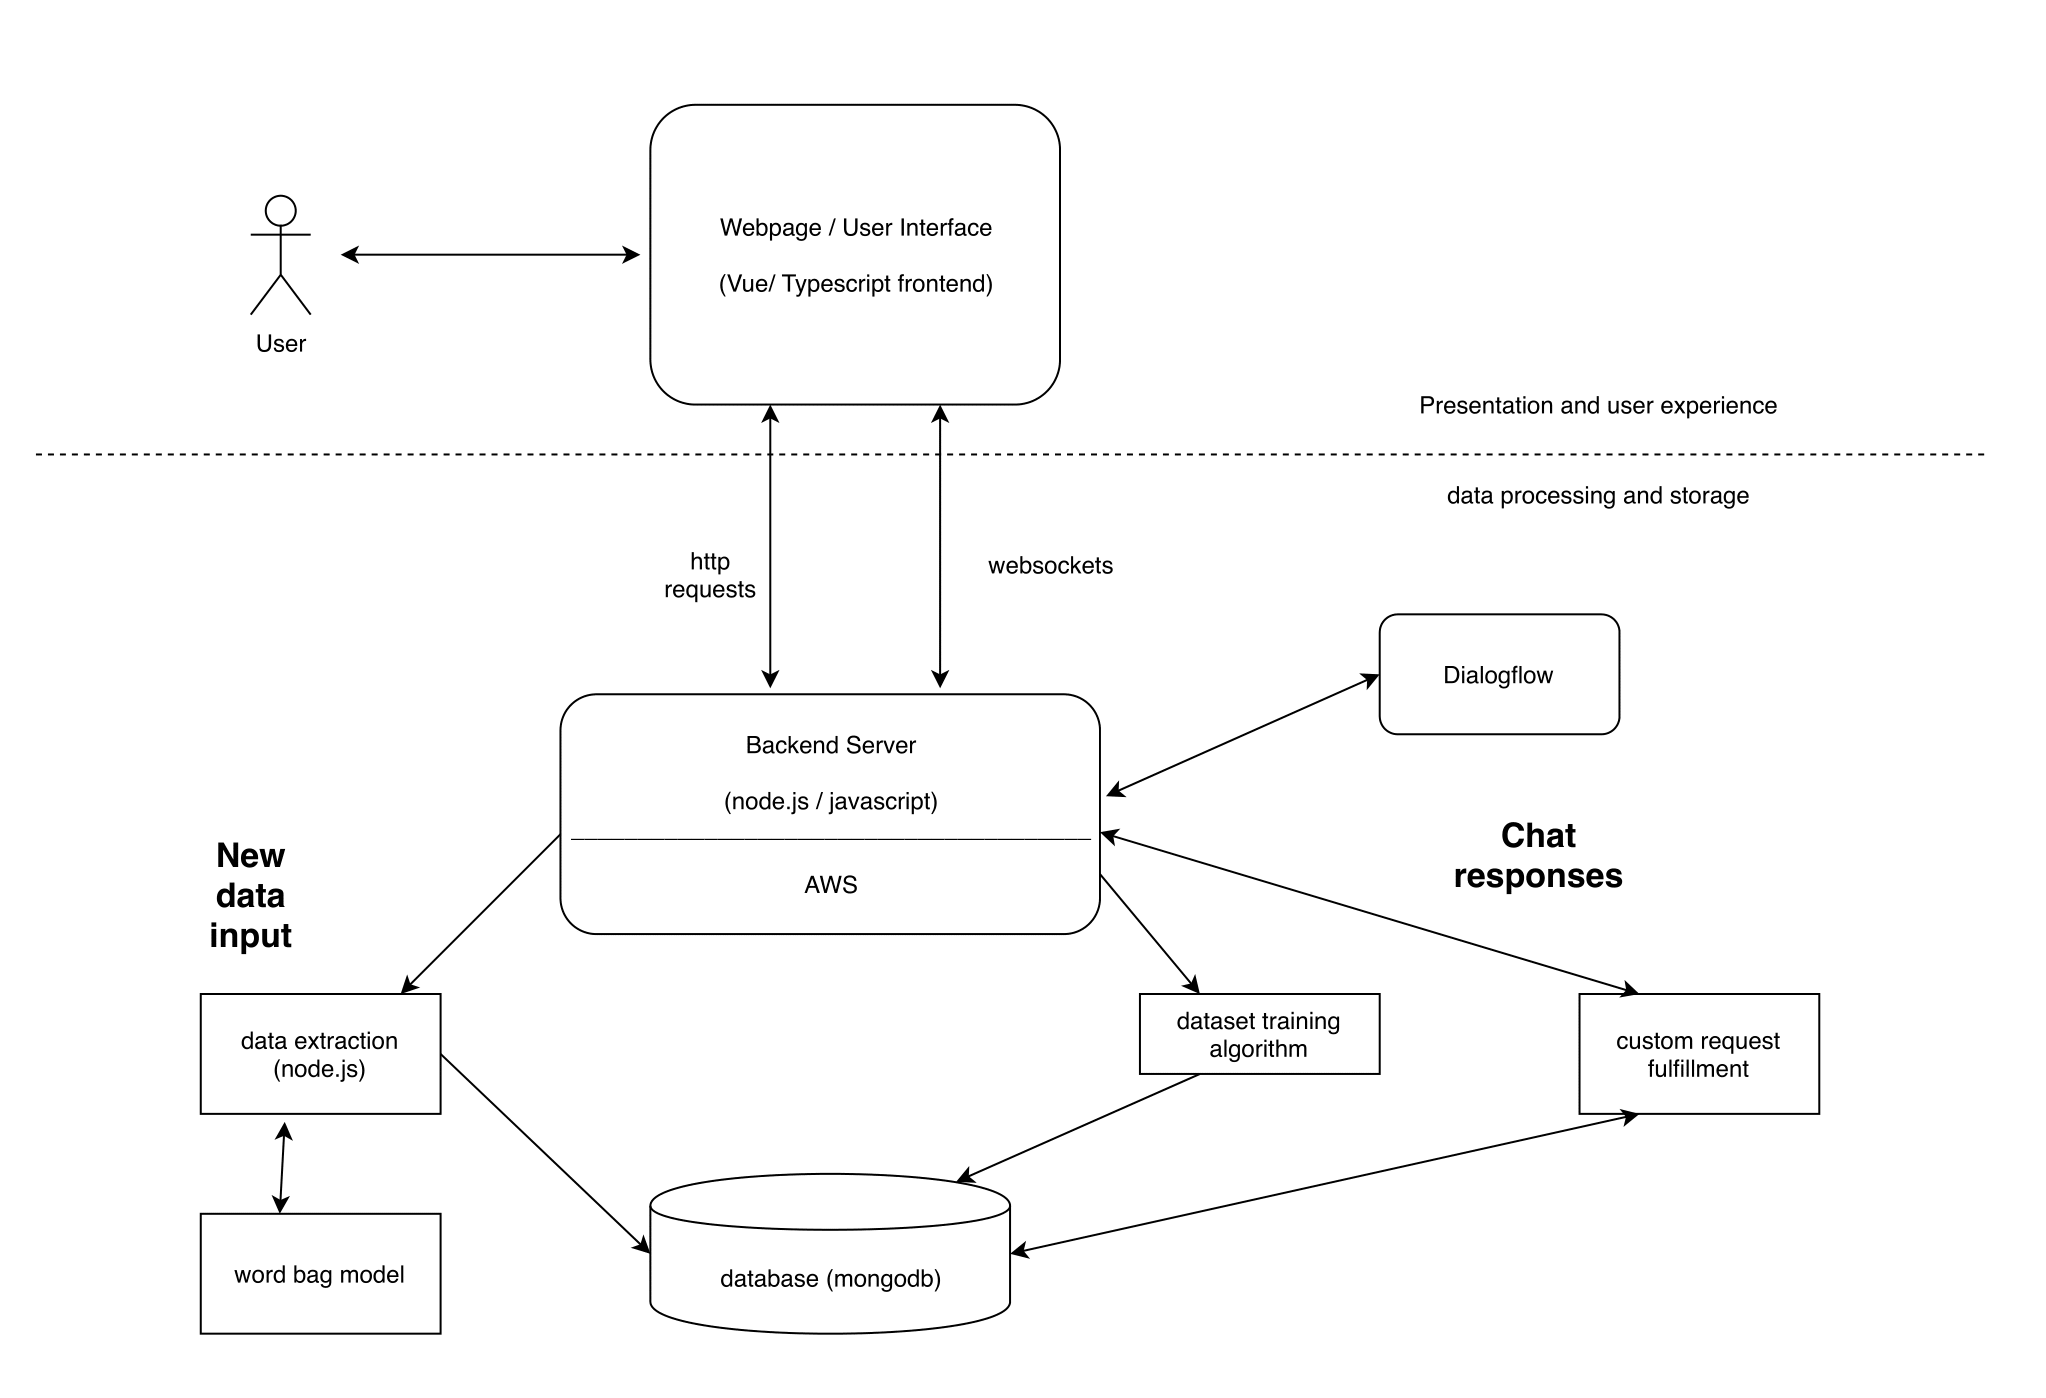
\includegraphics[width=\textwidth]{architecture-diagram.png}

\subsubsection{Data Scraping \& Processing}
The bot needs to be initialised when a new course is created. Without any initial data, it will take a significant amount of time before the bot has been trained to a sufficient degree such that it can give meaningful responses to students.

To solve this issue, we developed our own system to scrape and process the data on webcms3. There is a simple interface where the course administrator(s) can input the course code, name, forum and links to pages of content. Our data extraction module recursively follows these links to process and add the data to a database, to create an initial working data set.

It was necessary for us to build this component so that users could be onboarded with minimum hassle. This creates a very low barrier of entry, as the user only needs to provide a small amount of information, and the server will take care of the heavy lifting. Furthermore, webcms3 content is difficult to parse with prebuilt, generic web scraping tools due to its lack of ids and labels, hence the need to build our own tool from scratch.

\subsubsection{Extensible Backend}
Our bot was built entirely from scratch, with limited dependency on external APIs. The backend is responsible for a number of tasks, including but not limited to processing user queries, generating intelligent responses, managing user sessions and providing access to the relevant databases for user accounts and quiz questions. These tasks can be classfied into one of two loose categories: chat bot and internal API.

The chat bot is effectively the brain and bulk of our system, made to handle user queries. They are processed for keywords and intents to figure out what the user is asking about. Responses are generated accordingly, and are sent back to the user via the web interface, completing one iteration the interaction. This allows students to ask questions about the course content and logistics and receive correct information in a timely manner. The chat bot also provides the ability for students to ask for quizzes, which aid their study and help them revise with official, instructor-endorsed material.

The internal API is a subset of the backend that manages features that complement the functionality of the chat bot. Requests are made to the internal API on the backend via the frontend when the user interacts with the web interface. This enables features such as registering user accounts and adding quiz questions to the database. User state is managed to create personal instances of the bot for each student, which keeps track of frequent questions and problem areas. Adding quiz questions is part of the admin API, which gives course administrators the power to manage the bot for their course.

\subsubsection{Interactive User Interface}
As briefly mentioned in section 1.3.3, our frontend was built from the ground up. It was designed to be easy to use, aesthetically pleasing and extendable. To this end, we could develop additional features for our system that would not be possible if we were to use an existing chat platform, such as Facebook Messenger or Slack.

We have implemented a wide array of additional features that are only possible because of our custom frontend. For instance, the chat bot can ask for feedback on the quality of its response, and directly interact with the backend to adjust the weighting of the data in the database. It can also render tables and show images, and maintain a user state as mentioned in section 2.2.3.

Another section of our frontend is the administrator dashboard. This is the interface that allows course administrators to interact with the system and complete actions provided by the internal API. This includes inputting data (both to expand the bot's dataset, and in the form of quiz questions for students), as well as view information and statistics that the bot has collected.

\newpage
